\begin{figure*}[!t]
    \centering
    \begin{subfigure}[t]{2.3in}
        \centering
        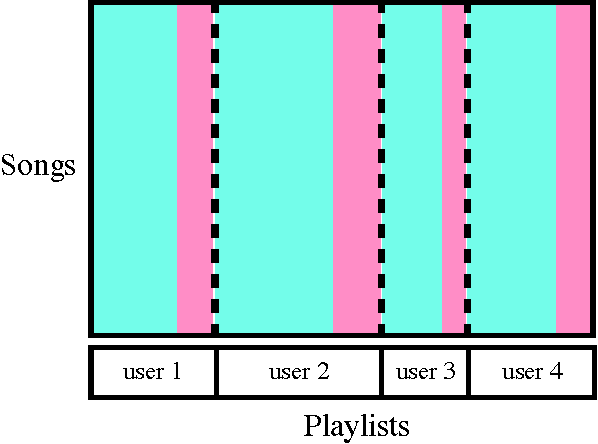
\includegraphics[height=1.6in]{fig/cp.pdf}
        \caption{Cold Playlists}
    \end{subfigure}
    \begin{subfigure}[t]{2.3in}
        \centering
        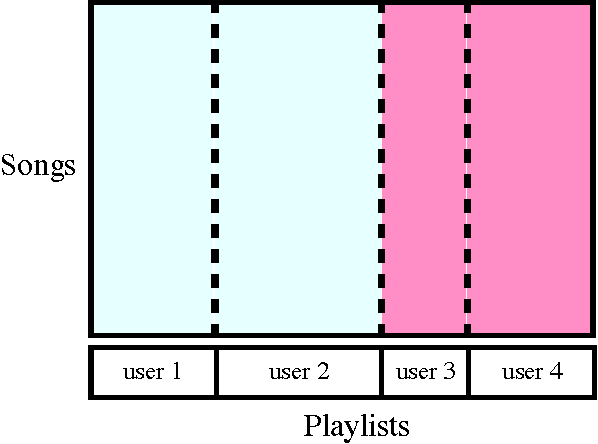
\includegraphics[height=1.6in]{fig/cu.pdf}
        \caption{Cold Users}
    \end{subfigure}
    \begin{subfigure}[t]{2.3in}
        \centering
        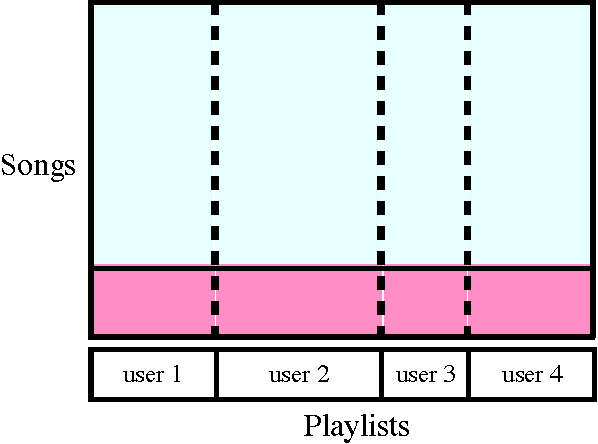
\includegraphics[height=1.6in]{fig/cs.pdf}
        \caption{Cold Songs}
    \end{subfigure}
    %\caption{Three cold-start settings: training set (cyan), test set (magenta)}
	\caption{Three settings of cold-start playlist recommendation.
In each setting,
rows represent songs, and a column represents a playlist, 
which is a binary vector where an element denotes if the corresponding song is in the playlist.
%Playlists are first grouped by user, then split into training (Cyan) and test set (Magenta).
%(a) Cold Playlists: a portion of playlists from each user are held for test
%See text below for description.
Playlists are grouped by user.
{\bf (a) Cold Playlists}: recommending personalised playlists (Magenta) for each user 
given users' existing playlists (Cyan); 
%by learning from her existing playlists (Cyan); 
{\bf (b) Cold Users}: recommending playlists for new users (Magenta) 
given playlists from existing users (Cyan);
%by learning playlists from existing users (Cyan); 
%by learning playlists from existing users (Cyan); 
{\bf (c) Cold Songs}: recommending newly released songs (Magenta) to extend users' existing playlists (Cyan).
}
\end{figure*}
